\documentclass[
    11pt,
    spanish,
	a4paper
]{article}
\usepackage[utf8]{inputenc}
\usepackage[spanish]{babel}
\usepackage{graphicx}
\usepackage{authoraftertitle}
\usepackage{float}
\usepackage{caption}
\usepackage{verbatim}
\usepackage{listings}
\captionsetup[table]{labelformat=empty}

\def\doctype{Trabajo práctico}
\title{Transformada de Fourier}
\author{Gonzalo Nahuel Vaca}

\begin{document}

\makeatletter
\begin{titlepage}
	\begin{center}
		\vspace*{1cm}
		
		\Huge
		\textbf{\doctype}
		\vspace{0.5cm}
    
		\LARGE
		\@title
		\vspace{0.5cm}
    
		\textbf{Procesamiento Digital de Señales (fundamentos)}
		
		\vspace{1.5cm}
		
		\textbf{\@author}

		\vspace{1.5cm}

		
\includegraphics[width=0.8\textwidth]{img/logoFIUBA.pdf}
		
		\vfill
		Maestría en Sistemas Embebidos\\
		Universidad de Buenos Aires\\
		Argentina\\
		\today
	\end{center}
\end{titlepage}
\makeatother
\newpage

\section{Parte 1}

\begin{lstlisting}[
    basicstyle=\tiny, %or \small or \footnotesize etc.
    ]
import numpy as np
import matplotlib.pyplot as plt
from scipy import signal


def sine(fs, f, amp, N, phase):
    t = np.arange(0, N / fs, 1 / fs)
    sig = amp * np.sin(2 * np.pi * f * t + phase)
    return sig


def square(fs, f, amp, N, phase):
    t = np.arange(0, N / fs, 1 / fs)
    sig = amp * signal.square(2 * np.pi * f * t + phase, duty=0.5)
    return sig


def sawtooth(fs, f, amp, N, phase):
    t = np.arange(0, N / fs, 1 / fs)
    sig = amp * signal.sawtooth(2 * np.pi * f * t + phase)
    return sig


def delta(N):
    # t = np.arange(0, N / fs, 1 / fs)
    sig = signal.unit_impulse(N)
    return sig


def powerAverage(signal):
    fft = np.fft.fft(signal) / len(signal)
    return np.sum(np.fft.fftshift(abs(fft)) ** 2)


if __name__ == "__main__":
    fs = 500
    f = 10
    N = 200
    phase = 0

    t = np.arange(0, N / fs, 1 / fs)
    nData = np.arange(0, N, 1)
    fData = nData * (fs / N) - (fs / 2)
    tf = np.arange(-fs / 2, (fs / 2) - (fs / N), fs / N)
    fig = plt.figure()

    sine = sine(fs, f, 1, N, phase)
    sineAxe = fig.add_subplot(4, 2, 1)
    plt.plot(t, sine, "b-", linewidth=1, alpha=1, label="Sine")
    plt.grid()
    plt.title(
        "Sine: f=10Hz, fs=500Hz, N=200, phase=0, powerAverage="
        + str(round(powerAverage(sine), 2))
        + "W"
    )
    sineFFTAxe = fig.add_subplot(4, 2, 2)
    sineFFTAxe.set_xlim(-fs / 2, (fs / 2) - (fs / N))
    plt.plot(fData, np.abs(np.fft.fftshift(np.fft.fft(sine)) / N) ** 2)
    plt.grid()
    plt.title("FFT(sine)")

    square = square(fs, f, 1, N, phase)
    squareAxe = fig.add_subplot(4, 2, 3)
    plt.plot(t, square, "b-", linewidth=1, alpha=1, label="Square")
    plt.grid()
    plt.title(
        "Square: f=10Hz, fs=500Hz, N=200, phase=0, powerAverage="
        + str(round(powerAverage(square), 2))
        + "W"
    )
    squareFFTAxe = fig.add_subplot(4, 2, 4)
    squareFFTAxe.set_xlim(-fs / 2, (fs / 2) - (fs / N))
    plt.plot(fData, np.abs(np.fft.fftshift(np.fft.fft(square)) / N) ** 2)
    plt.grid()
    plt.title("FFT(Square)")

    sawtooth = sawtooth(fs, f, 1, N, phase)
    squareAxe = fig.add_subplot(4, 2, 5)
    plt.plot(t, sawtooth, "b-", linewidth=1, alpha=1, label="Sawtooth")
    plt.grid()
    plt.title(
        "Sawtooth: f=10Hz, fs=500Hz, N=200, phase=0, powerAverage="
        + str(round(powerAverage(sawtooth), 2))
        + "W"
    )
    squareFFTAxe = fig.add_subplot(4, 2, 6)
    squareFFTAxe.set_xlim(-fs / 2, (fs / 2) - (fs / N))
    plt.plot(fData, np.abs(np.fft.fftshift(sawtooth) / N) ** 2)
    plt.grid()
    plt.title("FFT(Sawtooth)")
    # Delta plot
    delta = signal.unit_impulse(N)
    deltaAxe = fig.add_subplot(4, 2, 7)
    plt.plot(t, delta, "b-", linewidth=1, alpha=1, label="Delta")
    plt.grid()
    plt.title("Delta: t=0, powerAverage=" + str(round(powerAverage(sine), 2)) + "W")
    deltaFFTAxe = fig.add_subplot(4, 2, 8)
    deltaFFTAxe.set_xlim(-fs / 2, (fs / 2) - (fs / N))
    plt.plot(fData, np.abs(np.fft.fftshift(np.fft.fft(delta)) / N) ** 2)
    plt.grid()
    plt.title("FFT(Delta)")
    plt.show()
\end{lstlisting}

En la figura \ref{fig:parte1} se puede observar el funcionamiento del script.

\begin{figure}[htbp]
	\centering
	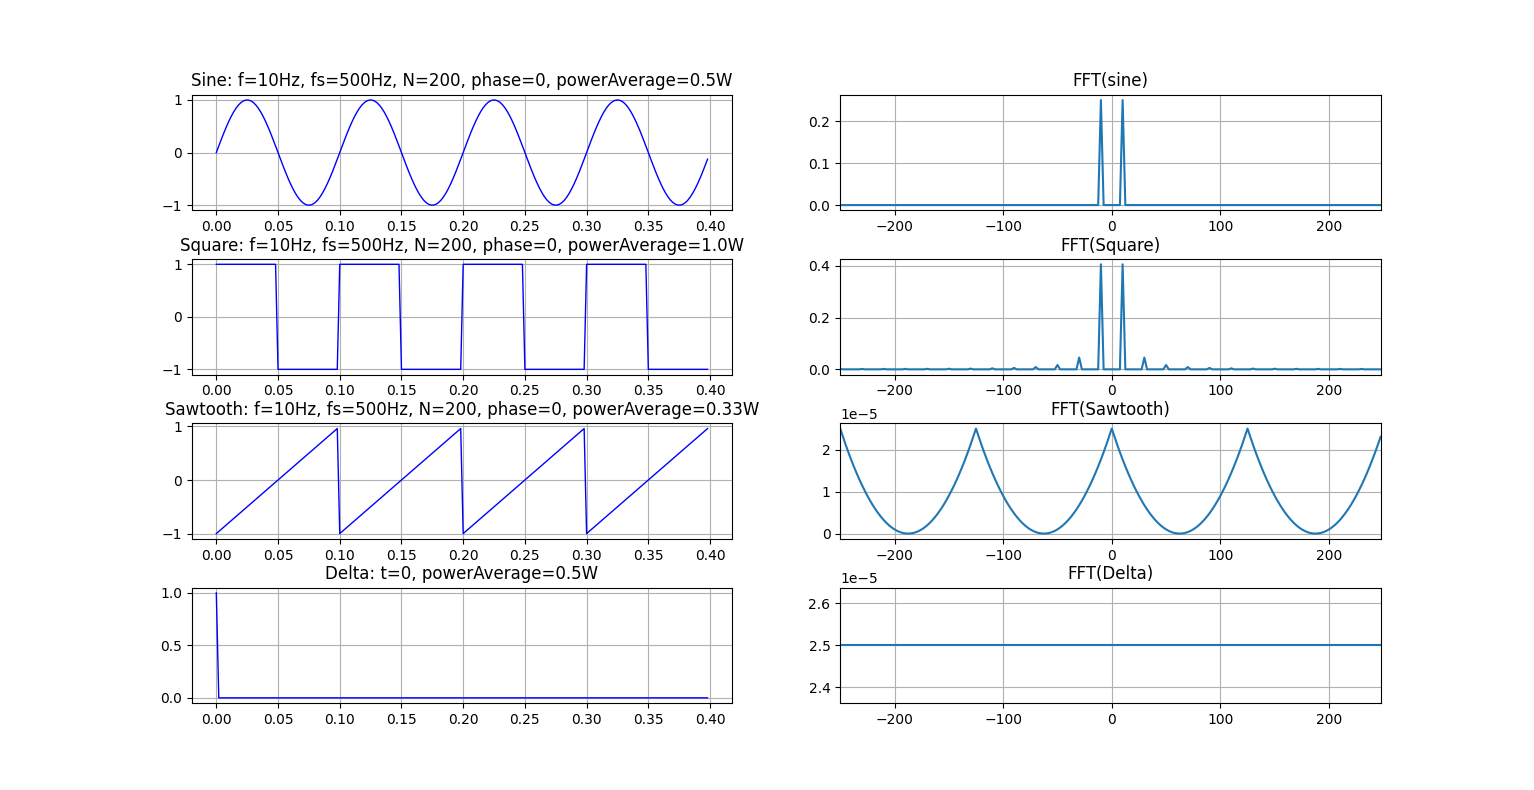
\includegraphics[width=\textwidth]{img/parte1.png}
	\caption{Imagen de las señales y sus transformadas.}
	\label{fig:parte1}
\end{figure}

\end{document}